\documentclass[11pt]{article}
\usepackage[utf8]{inputenc}
\usepackage[T1]{fontenc}
\usepackage{minted}
\usepackage{multirow}
\usepackage{enumerate}
\usepackage{tikz}

%% for listings..
\newminted{perl}{linenos, bgcolor=mintedBg, fontsize=\footnotesize}
\newminted{r}{linenos, bgcolor=mintedBg, fontsize=\footnotesize}
\definecolor{mintedBg}{rgb}{0.95, 0.95, 0.95}
\definecolor{blockBg}{rgb}{0.6, 0.6, 0.95}

\begin{document}

\section{Bioinformatics in General}
\begin{enumerate}
\item What is bioinformatics and why is it becoming an essential topic for
  biologists?\\
  Note that the there is no single correct answer to this question, and that
  you will not be judged on what you argue, but on how reasonable and informed
  your argument is.
  
  In your answer you may wish to consider the following:
  \begin{itemize}
  \item your opinion of what bioinformatics is
  \item the technologies or skills that are used within the field
  \item the impact of technological process on biological experiments
  \end{itemize}
  \item Describe some examples of problems and fields addressed by
    Bioinformatics. Full marks require at least three examples; points
    will be given both for depth of explanation and for numbers of points.
  \item Why is there such an emphasis of the analysis of sequences within
    bioinformatics? (Any reasonable answer will be accepted).
  \item Describe and contrast how genes were identified before and after the
    availability of cheap DNA sequencing.
  \item Why do we need sequences?
  \item Given an example of DNA sequence analysis that does not involve the
    alignment of sequences.
  \item What do we mean by, and when do we make use of sequence assembly?
  \item Give some examples of how we make use of sequence comparisons?
  \item What's the general relationship between sequence alignment and
    sequence comparison?
\end{enumerate}

\section{Molecular Biology \& the Central Dogma}  
\begin{enumerate}
\item Describe how information is stored, transmitted and made use of in biological
  systems. What are the important properties of the different types of
  macro-molecules used in this process?
  \begin{itemize}
    \item What is DNA?
    \item How does it differ from RNA?
    \item Why does this matter?
    \item How do proteins differ from nucleic acids?
    \item What do we mean when we say that two nucleic acid sequences (RNA or
      DNA) are complementary?
    \item The majority of DNA molecules are double stranded, whereas the
      majority of RNA molecules are single stranded. Discuss the impact of
      strandedness (consider replication / structural properties).
    \item What is this process generally called?
  \end{itemize}
\item Describe the structure of genes in both prokaryotes and
  eukaryotes. Include as many features as you can.
  \begin{itemize}
  \item How do we usually define a gene? (bonus points: How does this differ
    from the historical definition of a gene).
  \item For bonus points, discuss what should be included as part of a gene
    and how this makes it difficult to define the number of genes an organism
    has. 
  \end{itemize}
\item Give some exceptions to the Central Dogma.
\item What is the difference between RNA and DNA monomers?
\item How do the monomers of nucleic acids differ from those of proteins? How
  does this relate to their function?
\item What are exons and introns?
\item What is a codon? How long is it and why?
\item What do we mean when we talk about the degeneracy of the genetic code?
\item Given a genetic code:\\
  \begin{minipage}{0.6\textwidth}
  {\tiny
    %% this requires 
%% usepackage{multirow}
%% usepackage{tabularx}

\renewcommand{\arraystretch}{1.25}
\begin{tabular}{ |l| l l|l l| l l|l l|l| }
  \hline
  \multirow{2}{2em}{1st base} &
  \multicolumn{8}{|c|}{2nd base} &
  \multirow{2}{2em}{3rd base} \\
  \cline{2-9}
  &
  \multicolumn{2}{|c|}{U} &
  \multicolumn{2}{|c|}{C} &
  \multicolumn{2}{|c|}{A} &
  \multicolumn{2}{|c|}{G} & \\
  \hline
  \multirow{4}{2em}{U} & 
  UUU & \multirow{2}{4em}{\tiny (Phe/F)} &
  UCU & \multirow{4}{4em}{\tiny (Ser/S)} &
  UAU & \multirow{2}{4em}{\tiny (Tyr/Y)} &
  UGU & \multirow{2}{4em}{\tiny (Cys/C)} & U \\
  & UUC & & UCC & & UAC & & UGC & & C \\ \cline{2-3} \cline{6-9}
  & UUA & \multirow{6}{4em}{\tiny (Leu/L)} 
  & UCA & & UUA & Stop & UGA & (Stop) & A \\ \cline{8-9}
  & UUG & & UCG & & UAG & Stop & UGG & \tiny (Trp/W) & G \\ \cline{4-9} 
  \cline{1-1}
  \multirow{4}{2em}{C}
  & CUU & & CCU & \multirow{4}{4em}{(Pro/P)} & CAU & \multirow{2}{4em}{(His/H)} & CGU & \multirow{4}{4em}{(Arg/R)} & U \\
  & CUC & & CCC & & CAC & & CGC & & C \\ \cline{6-7}
  & CUA & & CCA & & CAA & \multirow{2}{4em}{Gln/Q} & CGA & & A \\
  & CUG & & CCG & & CAG & & CGG & & G \\ \cline{1-9}
  \multirow{4}{2em}{A}
  & AUU & \multirow{3}{4em}{(Ile/I)} & ACU & \multirow{4}{4em}{(Thr/T)} & AAU 
  & \multirow{2}{4em}{(Asn/N)} & AGU & \multirow{2}{4em}{(Ser/S)} & U \\
  & AUC & & ACC & & AAC & & AGC & & C \\ \cline{6-9}
  & AUA & & ACA & & AAA & \multirow{2}{4em}{(Lys/K)} & AGA & \multirow{2}{4em}{(Arg/R)} & A \\
  \cline{2-3}
  & AUG & (Met/M) & ACG & & AAG & & AGG & & G \\ \cline{1-9}
  \multirow{4}{4em}{G}
  & GUU & \multirow{4}{4em}{(Val/V)} & GCU & \multirow{4}{4em}{(Ala/A)} 
  & GAU & \multirow{2}{4em}{(Asp/D)} & GGU & \multirow{4}{4em}{(Gly/G)} & U \\
  & GUC & & GCC & & GAC & & GGC & & C \\ \cline{6-7}
  & GUA & & GCA & & GAA & \multirow{2}{4em}{(Glu/E)} & GGA & & A \\
  & GUG & & GCG & & GAG & & GGG & & G \\ \hline
\end{tabular}

  }
  \end{minipage}

  Give all the amino acide sequences that can be encoded by:\\
  \verb|ATCAGATAGATATTACCG|
\item What is an open reading frame (ORF)? What good are they to
  bioinformaticians?
\item What kind of mutations can arise in DNA sequences? What effects
  do the different types of mutations have on genes?
\end{enumerate}

\section{Biological databases}
\begin{enumerate}
\item Describe the typical structure of a web-facing databases. Comment on the
  different types of users and on how they use the database differently.
\item Describe examples of the types of data that is held in different
  databases. Comment on how the type of data affects how the data is stored
  and accessed.
\item Where can you find DNA sequences? (If you have trouble remembering
  specific names of databases, describe in some detail how you would go about finding a
  location / database that gives you DNA sequences).
\item How would you find biological information about a given DNA sequence?
  Include details about the type of information you can obtain from a DNA
  sequence and how this relates to the different types of DNA sequences
  (remember the structure of genes).
\item You search the [name witheld] database for a sequence representing a
  specific gene. You get several hundred sequences back. What is the reason
  for the multitude of sequences? What can you do to obtain only relevant
  sequences? Finally, what questions might you be able to address with the
  full set of sequences you obtained?
\item What are the differences between the Genbank, EMBL and DDBJ databases?
\item Describe the fasta sequence format.
\item Apart from sequence data what does the fastq format contain?
\item What are genome databases and why are they useful?
\end{enumerate}

\section{Pairwise alignment}
\begin{enumerate}
\item For the two sequences: \verb|5' TAATTAGC 3'| and \verb|5' CATTA 3'| :
  \begin{enumerate}
    \item Provide three reasonable alignments.
    \item Describe how you can score the alignments using sets of penalties
      (remember that you can have negative penalties).
    \item Score the alignments using at least two different sets of
      penalties. Comment on how the choice of penalties relates to the
      biological question being asked.
    \item Which of your alignments do you think is most reasonable and why? If you
      think all are equally reasonable then explain your opinion.
  \end{enumerate}
\item Why do we often use a different penalty for gap insertion and gap
  extension? Provide an example alignment with your question.
\item What's a dotplot? What can we use it for?
\item What do we mean by an optimal alignment?
\item What is the difference between a global and local alignment?
\item What is this?
  \begin{figure}[H]
    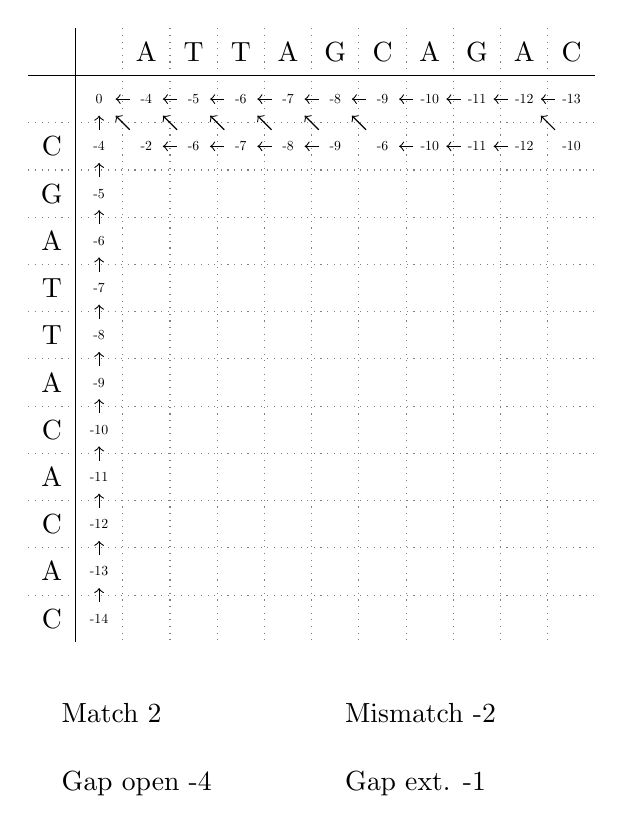
\begin{tikzpicture}[scale=0.6]
      \node [right] at (1,-1) {Match 2};
\node [right] at (7,-1) {Mismatch -2};
\node [right] at (1,-2.5) {Gap open -4};
\node [right] at (7,-2.5) {Gap ext. -1};


\draw [-] (0.5,12.5) -- (12.5,12.5);
\draw [-] (1.5,13.5) -- (1.5,0.5);
\draw [-, dotted, opacity=0.5] (0.5,11.5) -- (12.5,11.5);
\draw [-, dotted, opacity=0.5] (2.5,13.5) -- (2.5,0.5);
	\node at (3,13) {A};
	\draw [-, dotted, opacity=0.5] (3.5,13.5) -- (3.5,0.5);
	\node at (4,13) {T};
	\draw [-, dotted, opacity=0.5] (4.5,13.5) -- (4.5,0.5);
	\node at (5,13) {T};
	\draw [-, dotted, opacity=0.5] (5.5,13.5) -- (5.5,0.5);
	\node at (6,13) {A};
	\draw [-, dotted, opacity=0.5] (6.5,13.5) -- (6.5,0.5);
	\node at (7,13) {G};
	\draw [-, dotted, opacity=0.5] (7.5,13.5) -- (7.5,0.5);
	\node at (8,13) {C};
	\draw [-, dotted, opacity=0.5] (8.5,13.5) -- (8.5,0.5);
	\node at (9,13) {A};
	\draw [-, dotted, opacity=0.5] (9.5,13.5) -- (9.5,0.5);
	\node at (10,13) {G};
	\draw [-, dotted, opacity=0.5] (10.5,13.5) -- (10.5,0.5);
	\node at (11,13) {A};
	\draw [-, dotted, opacity=0.5] (11.5,13.5) -- (11.5,0.5);
	\node at (12,13) {C};
	\node at (1,11) {C};
	\draw [-, dotted, opacity=0.5] (0.5,10.5) -- (12.5,10.5);
	\node at (1,10) {G};
	\draw [-, dotted, opacity=0.5] (0.5,9.5) -- (12.5,9.5);
	\node at (1,9) {A};
	\draw [-, dotted, opacity=0.5] (0.5,8.5) -- (12.5,8.5);
	\node at (1,8) {T};
	\draw [-, dotted, opacity=0.5] (0.5,7.5) -- (12.5,7.5);
	\node at (1,7) {T};
	\draw [-, dotted, opacity=0.5] (0.5,6.5) -- (12.5,6.5);
	\node at (1,6) {A};
	\draw [-, dotted, opacity=0.5] (0.5,5.5) -- (12.5,5.5);
	\node at (1,5) {C};
	\draw [-, dotted, opacity=0.5] (0.5,4.5) -- (12.5,4.5);
	\node at (1,4) {A};
	\draw [-, dotted, opacity=0.5] (0.5,3.5) -- (12.5,3.5);
	\node at (1,3) {C};
	\draw [-, dotted, opacity=0.5] (0.5,2.5) -- (12.5,2.5);
	\node at (1,2) {A};
	\draw [-, dotted, opacity=0.5] (0.5,1.5) -- (12.5,1.5);
	\node at (1,1) {C};


	\node[scale=0.5] at (2,12) {0};
	\node[scale=0.5] at (3,12) {-4};
	\draw [->] (2.65, 11+1) -- (2.35, 11+1);
	\node[scale=0.5] at(4,12) {-5};
	\draw [->] (3.65,11+1) -- (3.35,11+1);
	\node[scale=0.5] at(5,12) {-6};
	\draw [->] (4.65,11+1) -- (4.35,11+1);
	\node[scale=0.5] at(6,12) {-7};
	\draw [->] (5.65,11+1) -- (5.35,11+1);
	\node[scale=0.5] at(7,12) {-8};
	\draw [->] (6.65,11+1) -- (6.35,11+1);
	\node[scale=0.5] at(8,12) {-9};
	\draw [->] (7.65,11+1) -- (7.35,11+1);
	\node[scale=0.5] at(9,12) {-10};
	\draw [->] (8.65,11+1) -- (8.35,11+1);
	\node[scale=0.5] at(10,12) {-11};
	\draw [->] (9.65,11+1) -- (9.35,11+1);
	\node[scale=0.5] at(11,12) {-12};
	\draw [->] (10.65,11+1) -- (10.35,11+1);
	\node[scale=0.5] at(12,12) {-13};
	\draw [->] (11.65,11+1) -- (11.35,11+1);
	\node[scale=0.5] at (2,11) {-4};
	\draw [->] (2,11 + 0.35) -- (2, 11 + 0.65);
	\node[scale=0.5] at(2,10) {-5};
	\draw [->] (2,11-1 + 0.35) -- (2, 11-1 + 0.65);
	\node[scale=0.5] at(2,9) {-6};
	\draw [->] (2,11-2 + 0.35) -- (2, 11-2 + 0.65);
	\node[scale=0.5] at(2,8) {-7};
	\draw [->] (2,11-3 + 0.35) -- (2, 11-3 + 0.65);
	\node[scale=0.5] at(2,7) {-8};
	\draw [->] (2,11-4 + 0.35) -- (2, 11-4 + 0.65);
	\node[scale=0.5] at(2,6) {-9};
	\draw [->] (2,11-5 + 0.35) -- (2, 11-5 + 0.65);
	\node[scale=0.5] at(2,5) {-10};
	\draw [->] (2,11-6 + 0.35) -- (2, 11-6 + 0.65);
	\node[scale=0.5] at(2,4) {-11};
	\draw [->] (2,11-7 + 0.35) -- (2, 11-7 + 0.65);
	\node[scale=0.5] at(2,3) {-12};
	\draw [->] (2,11-8 + 0.35) -- (2, 11-8 + 0.65);
	\node[scale=0.5] at(2,2) {-13};
	\draw [->] (2,11-9 + 0.35) -- (2, 11-9 + 0.65);
	\node[scale=0.5] at(2,1) {-14};
	\draw [->] (2,11-10 + 0.35) -- (2, 11-10 + 0.65);


	\node [scale=0.5] at (3,11) {-2};
	\draw [->] (2.65,11.35) -- (2.35,11.65);
	\node [scale=0.5] at (4,11) {-6};
	\draw [->] (3.65,11.35) -- (3.35,11.65);
	\draw [->] (3.65,11) -- (3.35,11);
	\node [scale=0.5] at (5,11) {-7};
	\draw [->] (4.65,11.35) -- (4.35,11.65);
	\draw [->] (4.65,11) -- (4.35,11);
	\node [scale=0.5] at (6,11) {-8};
	\draw [->] (5.65,11.35) -- (5.35,11.65);
	\draw [->] (5.65,11) -- (5.35,11);
	\node [scale=0.5] at (7,11) {-9};
	\draw [->] (6.65,11.35) -- (6.35,11.65);
	\draw [->] (6.65,11) -- (6.35,11);
	\node [scale=0.5] at (8,11) {-6};
	\draw [->] (7.65,11.35) -- (7.35,11.65);
	\node [scale=0.5] at (9,11) {-10};
	\draw [->] (8.65,11) -- (8.35,11);
	\node [scale=0.5] at (10,11) {-11};
	\draw [->] (9.65,11) -- (9.35,11);
	\node [scale=0.5] at (11,11) {-12};
	\draw [->] (10.65,11) -- (10.35,11);
	\node [scale=0.5] at (12,11) {-10};
	\draw [->] (11.65,11.35) -- (11.35,11.65);



    \end{tikzpicture}
  \end{figure}
  \begin{enumerate}
  \item Fill in the next row with both numbers and arrows.
  \item What can you obtain from this table after it is completely filled in?
  \end{enumerate}
\item Obtain all optimal alignments from the following table:
  \begin{figure}[H]
    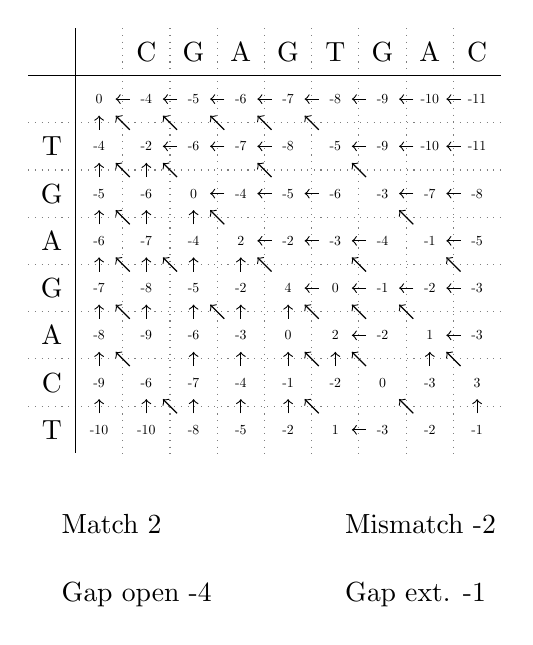
\begin{tikzpicture}[scale=0.6]
      \node [right] at (1,-1) {Match 2};
\node [right] at (7,-1) {Mismatch -2};
\node [right] at (1,-2.5) {Gap open -4};
\node [right] at (7,-2.5) {Gap ext. -1};

\draw [-] (0.5,8.5) -- (10.5,8.5);
\draw [-] (1.5,9.5) -- (1.5,0.5);
\draw [-, dotted, opacity=0.5] (0.5,7.5) -- (10.5,7.5);
\draw [-, dotted, opacity=0.5] (2.5,9.5) -- (2.5,0.5);
	\node at (3,9) {C};
	\draw [-, dotted, opacity=0.5] (3.5,9.5) -- (3.5,0.5);
	\node at (4,9) {G};
	\draw [-, dotted, opacity=0.5] (4.5,9.5) -- (4.5,0.5);
	\node at (5,9) {A};
	\draw [-, dotted, opacity=0.5] (5.5,9.5) -- (5.5,0.5);
	\node at (6,9) {G};
	\draw [-, dotted, opacity=0.5] (6.5,9.5) -- (6.5,0.5);
	\node at (7,9) {T};
	\draw [-, dotted, opacity=0.5] (7.5,9.5) -- (7.5,0.5);
	\node at (8,9) {G};
	\draw [-, dotted, opacity=0.5] (8.5,9.5) -- (8.5,0.5);
	\node at (9,9) {A};
	\draw [-, dotted, opacity=0.5] (9.5,9.5) -- (9.5,0.5);
	\node at (10,9) {C};
	\node at (1,7) {T};
	\draw [-, dotted, opacity=0.5] (0.5,6.5) -- (10.5,6.5);
	\node at (1,6) {G};
	\draw [-, dotted, opacity=0.5] (0.5,5.5) -- (10.5,5.5);
	\node at (1,5) {A};
	\draw [-, dotted, opacity=0.5] (0.5,4.5) -- (10.5,4.5);
	\node at (1,4) {G};
	\draw [-, dotted, opacity=0.5] (0.5,3.5) -- (10.5,3.5);
	\node at (1,3) {A};
	\draw [-, dotted, opacity=0.5] (0.5,2.5) -- (10.5,2.5);
	\node at (1,2) {C};
	\draw [-, dotted, opacity=0.5] (0.5,1.5) -- (10.5,1.5);
	\node at (1,1) {T};


	\node[scale=0.5] at (2,8) {0};
	\node[scale=0.5] at (3,8) {-4};
	\draw [->] (2.65, 7+1) -- (2.35, 7+1);
	\node[scale=0.5] at(4,8) {-5};
	\draw [->] (3.65,7+1) -- (3.35,7+1);
	\node[scale=0.5] at(5,8) {-6};
	\draw [->] (4.65,7+1) -- (4.35,7+1);
	\node[scale=0.5] at(6,8) {-7};
	\draw [->] (5.65,7+1) -- (5.35,7+1);
	\node[scale=0.5] at(7,8) {-8};
	\draw [->] (6.65,7+1) -- (6.35,7+1);
	\node[scale=0.5] at(8,8) {-9};
	\draw [->] (7.65,7+1) -- (7.35,7+1);
	\node[scale=0.5] at(9,8) {-10};
	\draw [->] (8.65,7+1) -- (8.35,7+1);
	\node[scale=0.5] at(10,8) {-11};
	\draw [->] (9.65,7+1) -- (9.35,7+1);
	\node[scale=0.5] at (2,7) {-4};
	\draw [->] (2,7 + 0.35) -- (2, 7 + 0.65);
	\node[scale=0.5] at(2,6) {-5};
	\draw [->] (2,7-1 + 0.35) -- (2, 7-1 + 0.65);
	\node[scale=0.5] at(2,5) {-6};
	\draw [->] (2,7-2 + 0.35) -- (2, 7-2 + 0.65);
	\node[scale=0.5] at(2,4) {-7};
	\draw [->] (2,7-3 + 0.35) -- (2, 7-3 + 0.65);
	\node[scale=0.5] at(2,3) {-8};
	\draw [->] (2,7-4 + 0.35) -- (2, 7-4 + 0.65);
	\node[scale=0.5] at(2,2) {-9};
	\draw [->] (2,7-5 + 0.35) -- (2, 7-5 + 0.65);
	\node[scale=0.5] at(2,1) {-10};
	\draw [->] (2,7-6 + 0.35) -- (2, 7-6 + 0.65);


	\node [scale=0.5] at (3,7) {-2};
	\draw [->] (2.65,7.35) -- (2.35,7.65);
	\node [scale=0.5] at (4,7) {-6};
	\draw [->] (3.65,7.35) -- (3.35,7.65);
	\draw [->] (3.65,7) -- (3.35,7);
	\node [scale=0.5] at (5,7) {-7};
	\draw [->] (4.65,7.35) -- (4.35,7.65);
	\draw [->] (4.65,7) -- (4.35,7);
	\node [scale=0.5] at (6,7) {-8};
	\draw [->] (5.65,7.35) -- (5.35,7.65);
	\draw [->] (5.65,7) -- (5.35,7);
	\node [scale=0.5] at (7,7) {-5};
	\draw [->] (6.65,7.35) -- (6.35,7.65);
	\node [scale=0.5] at (8,7) {-9};
	\draw [->] (7.65,7) -- (7.35,7);
	\node [scale=0.5] at (9,7) {-10};
	\draw [->] (8.65,7) -- (8.35,7);
	\node [scale=0.5] at (10,7) {-11};
	\draw [->] (9.65,7) -- (9.35,7);


	\node [scale=0.5] at (3,6) {-6};
	\draw [->] (2.65,6.35) -- (2.35,6.65);
	\draw [->] (3,6.35) -- (3,6.65);
	\node [scale=0.5] at (4,6) {0};
	\draw [->] (3.65,6.35) -- (3.35,6.65);
	\node [scale=0.5] at (5,6) {-4};
	\draw [->] (4.65,6) -- (4.35,6);
	\node [scale=0.5] at (6,6) {-5};
	\draw [->] (5.65,6.35) -- (5.35,6.65);
	\draw [->] (5.65,6) -- (5.35,6);
	\node [scale=0.5] at (7,6) {-6};
	\draw [->] (6.65,6) -- (6.35,6);
	\node [scale=0.5] at (8,6) {-3};
	\draw [->] (7.65,6.35) -- (7.35,6.65);
	\node [scale=0.5] at (9,6) {-7};
	\draw [->] (8.65,6) -- (8.35,6);
	\node [scale=0.5] at (10,6) {-8};
	\draw [->] (9.65,6) -- (9.35,6);


	\node [scale=0.5] at (3,5) {-7};
	\draw [->] (2.65,5.35) -- (2.35,5.65);
	\draw [->] (3,5.35) -- (3,5.65);
	\node [scale=0.5] at (4,5) {-4};
	\draw [->] (4,5.35) -- (4,5.65);
	\node [scale=0.5] at (5,5) {2};
	\draw [->] (4.65,5.35) -- (4.35,5.65);
	\node [scale=0.5] at (6,5) {-2};
	\draw [->] (5.65,5) -- (5.35,5);
	\node [scale=0.5] at (7,5) {-3};
	\draw [->] (6.65,5) -- (6.35,5);
	\node [scale=0.5] at (8,5) {-4};
	\draw [->] (7.65,5) -- (7.35,5);
	\node [scale=0.5] at (9,5) {-1};
	\draw [->] (8.65,5.35) -- (8.35,5.65);
	\node [scale=0.5] at (10,5) {-5};
	\draw [->] (9.65,5) -- (9.35,5);


	\node [scale=0.5] at (3,4) {-8};
	\draw [->] (2.65,4.35) -- (2.35,4.65);
	\draw [->] (3,4.35) -- (3,4.65);
	\node [scale=0.5] at (4,4) {-5};
	\draw [->] (3.65,4.35) -- (3.35,4.65);
	\draw [->] (4,4.35) -- (4,4.65);
	\node [scale=0.5] at (5,4) {-2};
	\draw [->] (5,4.35) -- (5,4.65);
	\node [scale=0.5] at (6,4) {4};
	\draw [->] (5.65,4.35) -- (5.35,4.65);
	\node [scale=0.5] at (7,4) {0};
	\draw [->] (6.65,4) -- (6.35,4);
	\node [scale=0.5] at (8,4) {-1};
	\draw [->] (7.65,4.35) -- (7.35,4.65);
	\draw [->] (7.65,4) -- (7.35,4);
	\node [scale=0.5] at (9,4) {-2};
	\draw [->] (8.65,4) -- (8.35,4);
	\node [scale=0.5] at (10,4) {-3};
	\draw [->] (9.65,4.35) -- (9.35,4.65);
	\draw [->] (9.65,4) -- (9.35,4);


	\node [scale=0.5] at (3,3) {-9};
	\draw [->] (2.65,3.35) -- (2.35,3.65);
	\draw [->] (3,3.35) -- (3,3.65);
	\node [scale=0.5] at (4,3) {-6};
	\draw [->] (4,3.35) -- (4,3.65);
	\node [scale=0.5] at (5,3) {-3};
	\draw [->] (4.65,3.35) -- (4.35,3.65);
	\draw [->] (5,3.35) -- (5,3.65);
	\node [scale=0.5] at (6,3) {0};
	\draw [->] (6,3.35) -- (6,3.65);
	\node [scale=0.5] at (7,3) {2};
	\draw [->] (6.65,3.35) -- (6.35,3.65);
	\node [scale=0.5] at (8,3) {-2};
	\draw [->] (7.65,3.35) -- (7.35,3.65);
	\draw [->] (7.65,3) -- (7.35,3);
	\node [scale=0.5] at (9,3) {1};
	\draw [->] (8.65,3.35) -- (8.35,3.65);
	\node [scale=0.5] at (10,3) {-3};
	\draw [->] (9.65,3) -- (9.35,3);


	\node [scale=0.5] at (3,2) {-6};
	\draw [->] (2.65,2.35) -- (2.35,2.65);
	\node [scale=0.5] at (4,2) {-7};
	\draw [->] (4,2.35) -- (4,2.65);
	\node [scale=0.5] at (5,2) {-4};
	\draw [->] (5,2.35) -- (5,2.65);
	\node [scale=0.5] at (6,2) {-1};
	\draw [->] (6,2.35) -- (6,2.65);
	\node [scale=0.5] at (7,2) {-2};
	\draw [->] (6.65,2.35) -- (6.35,2.65);
	\draw [->] (7,2.35) -- (7,2.65);
	\node [scale=0.5] at (8,2) {0};
	\draw [->] (7.65,2.35) -- (7.35,2.65);
	\node [scale=0.5] at (9,2) {-3};
	\draw [->] (9,2.35) -- (9,2.65);
	\node [scale=0.5] at (10,2) {3};
	\draw [->] (9.65,2.35) -- (9.35,2.65);


	\node [scale=0.5] at (3,1) {-10};
	\draw [->] (3,1.35) -- (3,1.65);
	\node [scale=0.5] at (4,1) {-8};
	\draw [->] (3.65,1.35) -- (3.35,1.65);
	\draw [->] (4,1.35) -- (4,1.65);
	\node [scale=0.5] at (5,1) {-5};
	\draw [->] (5,1.35) -- (5,1.65);
	\node [scale=0.5] at (6,1) {-2};
	\draw [->] (6,1.35) -- (6,1.65);
	\node [scale=0.5] at (7,1) {1};
	\draw [->] (6.65,1.35) -- (6.35,1.65);
	\node [scale=0.5] at (8,1) {-3};
	\draw [->] (7.65,1) -- (7.35,1);
	\node [scale=0.5] at (9,1) {-2};
	\draw [->] (8.65,1.35) -- (8.35,1.65);
	\node [scale=0.5] at (10,1) {-1};
	\draw [->] (10,1.35) -- (10,1.65);


    \end{tikzpicture}
  \end{figure}
  \begin{enumerate}
  \item Draw the process directly on the table.
  \item What kind of alignment(s) did you obtain?
  \end{enumerate}
\item How would you modify the Needleman-Wunsch (global alignment) to
  obtain a local alignment (Smith-Waterman)?
\item Fill in the first two rows and the first column of the following
  alignment table for a local alignment (Smith-Waterman).
  \begin{figure}[H]
    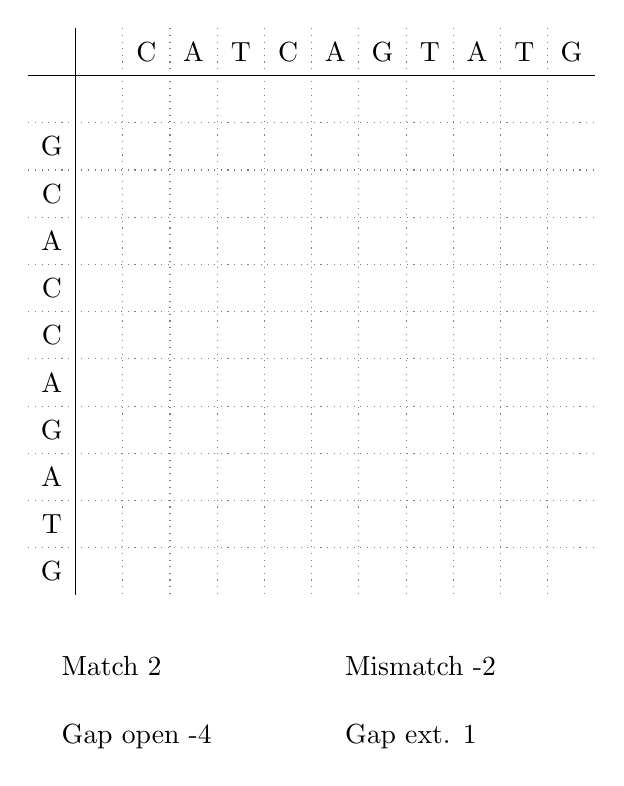
\begin{tikzpicture}[scale=0.6]
      \node [right] at (1,-1) {Match 2};
\node [right] at (7,-1) {Mismatch -2};
\node [right] at (1,-2.5) {Gap open -4};
\node [right] at (7,-2.5) {Gap ext. 1};

\draw [-] (0.5,11.5) -- (12.5,11.5);
\draw [-] (1.5,12.5) -- (1.5,0.5);
\draw [-, dotted, opacity=0.5] (0.5,10.5) -- (12.5,10.5);
\draw [-, dotted, opacity=0.5] (2.5,12.5) -- (2.5,0.5);
	\node at (3,12) {C};
	\draw [-, dotted, opacity=0.5] (3.5,12.5) -- (3.5,0.5);
	\node at (4,12) {A};
	\draw [-, dotted, opacity=0.5] (4.5,12.5) -- (4.5,0.5);
	\node at (5,12) {T};
	\draw [-, dotted, opacity=0.5] (5.5,12.5) -- (5.5,0.5);
	\node at (6,12) {C};
	\draw [-, dotted, opacity=0.5] (6.5,12.5) -- (6.5,0.5);
	\node at (7,12) {A};
	\draw [-, dotted, opacity=0.5] (7.5,12.5) -- (7.5,0.5);
	\node at (8,12) {G};
	\draw [-, dotted, opacity=0.5] (8.5,12.5) -- (8.5,0.5);
	\node at (9,12) {T};
	\draw [-, dotted, opacity=0.5] (9.5,12.5) -- (9.5,0.5);
	\node at (10,12) {A};
	\draw [-, dotted, opacity=0.5] (10.5,12.5) -- (10.5,0.5);
	\node at (11,12) {T};
	\draw [-, dotted, opacity=0.5] (11.5,12.5) -- (11.5,0.5);
	\node at (12,12) {G};
	\node at (1,10) {G};
	\draw [-, dotted, opacity=0.5] (0.5,9.5) -- (12.5,9.5);
	\node at (1,9) {C};
	\draw [-, dotted, opacity=0.5] (0.5,8.5) -- (12.5,8.5);
	\node at (1,8) {A};
	\draw [-, dotted, opacity=0.5] (0.5,7.5) -- (12.5,7.5);
	\node at (1,7) {C};
	\draw [-, dotted, opacity=0.5] (0.5,6.5) -- (12.5,6.5);
	\node at (1,6) {C};
	\draw [-, dotted, opacity=0.5] (0.5,5.5) -- (12.5,5.5);
	\node at (1,5) {A};
	\draw [-, dotted, opacity=0.5] (0.5,4.5) -- (12.5,4.5);
	\node at (1,4) {G};
	\draw [-, dotted, opacity=0.5] (0.5,3.5) -- (12.5,3.5);
	\node at (1,3) {A};
	\draw [-, dotted, opacity=0.5] (0.5,2.5) -- (12.5,2.5);
	\node at (1,2) {T};
	\draw [-, dotted, opacity=0.5] (0.5,1.5) -- (12.5,1.5);
	\node at (1,1) {G};



    \end{tikzpicture}
  \end{figure}
\item What is an amino acid substitution matrix and how would you use one?
\item Describe at least two ways in which you can derive an amino acid
  substitution matrix?
\item On what basis could you define a nucleotide substitution matrix for
  aligning DNA sequences?
\item The following is an example of an amino acid substitution table.
  \begin{figure}[H]
    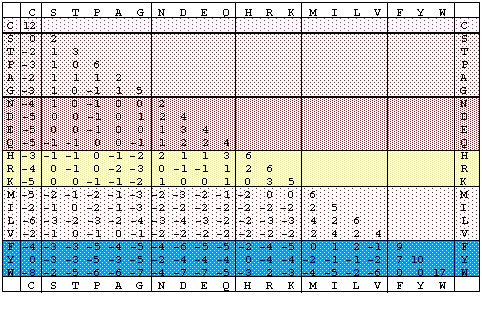
\includegraphics[width=0.7\textwidth]{images/dayhoff_256}
  \end{figure}
  \begin{enumerate}
  \item The table has high and low values. What do these mean?
  \item What do the numbers along the diagonal indicate? Why do they
    vary?
  \end{enumerate}
\end{enumerate}
  
\section{Multiple sequence alignment}
\begin{enumerate}
\item What are homologues, orthologues and paralogues?
\item Describe some uses of multiple sequence alignment.
\item What are heuristic methods? Why do we use them?
\item What are the three steps of the Clustal method?
\item How does the Clustal method make use of a guide tree?
\item Describe a simple method to obtain a guide tree.
\end{enumerate}

\section{Perl}
\begin{enumerate}
\item What is Perl, and what is it useful for?
\item What are the three ways in which you can store values in Perl? Give
  examples as to how you can assign values to such variables?
\item What does the following code do?

  \begin{perlcode}
    #!/usr/bin/perl -w
    
    $a = $ARGV[0];
    $b = $ARGV[1];

    print "$a + $b = ", $a + $b, "\n";
    
  \end{perlcode}
  Explain what kind of errors you may get running the above code.
\item What does the following code do?

  \begin{perlcode}
    #!/usr/bin/perl -w

    @a = (0,1);
    for($i = 2; $i < 100; $i++){
      $a[$i] = $a[$i-2] + $a[$i-1];
    }
    
    for $v(@a){
      print "$v\n";
    }
    \end{perlcode}
\item The Fibonacci sequence is defined as a sequence of numbers starting
  with 1,1 or 0,1 and where every subsequent number is the sum of the two
  previous numbers. That is: $F_i = F_{i-2} + F_{i-1}$. Write a small piece
  of Perl that calculates and prints the first 100 values of the Fibonacci
  sequence.
\item How would you represent a table of values in Perl?
\item Why is the following problematic:

  \begin{perlcode}
    $v1 = "one";
    $v2 = 2;
    $v3 = $v1 + $v2;
  \end{perlcode}
\item What is the difference between:

  \begin{perlcode}
    if($a eq $b)
  \end{perlcode}
  and

  \begin{perlcode}
    if($a == $b)
  \end{perlcode}
  When would you use one rather than the other?
\item What will the following code print:

  \begin{perlcode}
  $a = 10;
  $b = 8;
  if($b = $a){
    print "$a is equal to $b\n";
  }else{
    print "$a is not equal to $b\n";
  }
  \end{perlcode}
  Read carefullly; there is a small trick here.
\end{enumerate}

\end{document}
